\section{Phương pháp và kiến trúc nghiên cứu}
\label{sec:methodology_architecture}

\subsection{Phát biểu Bài toán và Mục tiêu Tối ưu hóa}
Bài toán STLF được phát biểu dưới dạng hồi quy chuỗi thời gian có biến ngoại sinh. Tại mỗi bước thời gian giờ $t \in \{1, \dots, T\}$, hệ thống nhận vector đặc trưng đầu vào $\mathbf{x}_t \in \mathbb{R}^D$ và dự báo phụ tải thực tế $y_t \in \mathbb{R}^+$ (MW):
\begin{equation}
    \mathbf{x}_t = \left[ \mathbf{x}_t^{\text{temporal}}, \, \mathbf{x}_t^{\text{weather}}, \, \mathbf{x}_t^{\text{dynamics}}, \, \mathbf{x}_t^{\text{physics}} \right]^T \in \mathbb{R}^D
\end{equation}
Mục tiêu là tìm hàm ánh xạ $f^* \in \mathcal{F}$ cực tiểu hóa sai số toàn phương trung bình:
\begin{equation}
    f^* = \argmin_{f \in \mathcal{F}} \; \mathbb{E}_{(\mathbf{x}_t, y_t) \sim \mathcal{D}} \left[ \big(y_t - f(\mathbf{x}_t)\big)^2 \right]
\end{equation}

\subsection{Phương pháp Đối chuẩn (Baseline)}
Nghiên cứu kế thừa baseline hàng đầu của Roy et al.~\cite{roy2025hourly}: mô hình 24-Hourly XGBoost phân đoạn theo 24 giờ trong ngày. Trong baseline này, mỗi giờ $h \in \{1, \dots, 24\}$ được huấn luyện một cây XGBoost độc lập với các biến trích xuất từ 5 trạm nhiệt độ và 5 trạm bức xạ mặt trời qua PCA cùng biến trễ động học 1 giờ ($\text{PCA\_Temp\_Lag1}$).

\subsection{Kiến trúc Khung Phương pháp Đề xuất}
Kiến trúc tổng thể của nghiên cứu được tổ chức theo pipeline nghiên cứu khép kín gồm 5 giai đoạn liên hoàn (Hình~\ref{fig:pipeline_architecture}):
\begin{center}
\textbf{Input Data} $\to$ \textbf{PCA Preprocessing} $\to$ \textbf{Physics Features} $\to$ \textbf{Dual Base Models} $\to$ \textbf{Context-Aware Meta-Learner} $\to$ \textbf{Evaluation}
\end{center}

\begin{figure}[htbp]
    \centering
    \begin{tcolorbox}[colback=gray!5,colframe=aivnGreen,arc=3mm,boxrule=0.8pt,width=0.98\linewidth,title={\bfseries Sơ đồ Kiến trúc Pipeline: Context-Aware Dual-Regime Stacking (CAS)},fonttitle=\sffamily\bfseries]
    \centering
    \small
    \begin{verbatim}
┌────────────────────────────────────────────────────────────────────────────────────────┐
│                               1. DỮ LIỆU ĐẦU VÀO NGOẠI SINH                            │
│    5 Trạm Quan trắc Nhiệt độ (T1..T5)      5 Trạm Quan trắc Bức xạ Mặt trời (G1..G5)   │
└───────────────────────────┬────────────────────────────────┬───────────────────────────┘
                            │                                │
                 ┌──────────▼──────────┐          ┌──────────▼──────────┐
                 │  PCA Giảm Chiều Temp│          │  PCA Giảm Chiều GHI │
                 │    (VIF: 48.8 -> 2.47)│        │   (VIF: 1055 -> 2.07)│
                 └──────────┬──────────┘          └──────────┬──────────┘
                            │                                │
                            ▼                                ▼
┌────────────────────────────────────────────────────────────────────────────────────────┐
│                        2. KỸ NGHỆ ĐẶC TRƯNG ĐỊNH HƯỚNG VẬT LÝ                          │
│   • Physics HVAC: Heating / Cooling Degree Days (HDD & CDD tại ngưỡng cơ sở 18°C)      │
│   • Chu kỳ Sóng Fourier liên tục: Sin/Cos(DOY / 365.25) & Sin/Cos(Hour / 24)           │
│   • Biến động học trễ thời gian: PCA_Temp_Lag1, PCA_GHI_Lag1                           │
└───────────────────────────┬────────────────────────────────┬───────────────────────────┘
                            │                                │
                 ┌──────────▼──────────┐          ┌──────────▼──────────┐
                 │  Base Model 1       │          │  Base Model 2       │
                 │  ElasticNet (Linear,│          │  XGBoost (Non-linear│
                 │   Nocturnal Baseload│          │   Trees, Peak Load) │
                 └──────────┬──────────┘          └──────────┬──────────┘
                            │ ŷ_linear                       │ ŷ_tree
                            └───────────────┬────────────────┘
                                            │
                                            ▼
┌────────────────────────────────────────────────────────────────────────────────────────┐
│                   3. CONTEXT-AWARE META-LEARNER (LIGHTGBM - CAS)                       │
│                                                                                        │
│   Vector Đầu vào Ghép nối: [ŷ_linear, ŷ_tree]  +  [Hour, HDD, CDD, Fourier, Weather]   │
│                                                                                        │
│   • Ban đêm (00:00 - 06:00): Tự động ưu tiên trọng số dự báo của ElasticNet            │
│   • Sóng nhiệt (CDD > 3°C) : Tự động định tuyến chuyển quyền cho XGBoost               │
└───────────────────────────────────────────┬────────────────────────────────────────────┘
                                            │
                                            ▼
                                 DỰ BÁO PHỤ TẢI CUỐI CÙNG
    \end{verbatim}
    \end{tcolorbox}
    \caption{Sơ đồ pipeline phương pháp Context-Aware Dual-Regime Stacking (CAS) tích hợp tri thức vật lý.}
    \label{fig:pipeline_architecture}
\end{figure}

\subsubsection{1. Khử Đa cộng tuyến Ngoại sinh bằng PCA}
Để định lượng đa cộng tuyến giữa 5 trạm quan trắc nhiệt độ và 5 trạm bức xạ, chỉ số phóng đại phương sai (\textit{Variance Inflation Factor} -- VIF) được tính toán: $\text{VIF}_j = 1 / (1 - R_j^2)$. Bảng~\ref{tab:vif_analysis} chứng minh rằng trước PCA, chỉ số VIF bùng nổ lên tới $52.70$ (nhiệt độ) và $1055.70$ (bức xạ mặt trời). Sau khi chiếu PCA, thành phần chính thứ nhất $\text{PCA\_Temp}$ giải thích $>91.5\%$ phương sai với $\text{VIF} = \mathbf{2.47}$, và $\text{PCA\_GHI}$ giải thích $>88.2\%$ phương sai với $\text{VIF} = \mathbf{2.07}$ (Hình~\ref{fig:pca_variance}), loại bỏ hoàn toàn nguy cơ bất ổn định số học.

\begin{table}[htbp]
    \centering
    \caption{Chỉ số VIF của các trạm đo nhiệt độ và bức xạ mặt trời trước và sau khi áp dụng PCA.}
    \label{tab:vif_analysis}
    \begin{tabular}{lc|lc|lc}
        \toprule
        \multicolumn{2}{c|}{\textbf{Nhiệt độ (Trước PCA)}} & \multicolumn{2}{c|}{\textbf{Bức xạ GHI (Trước PCA)}} & \multicolumn{2}{c}{\textbf{Sau khi Áp dụng PCA}} \\
        \textbf{Biến trạm đo} & \textbf{VIF} & \textbf{Biến trạm đo} & \textbf{VIF} & \textbf{Biến tổng hợp} & \textbf{VIF} \\
        \midrule
        Site-1 Temp & 31.74 & Site-1 GHI & 180.98 & PCA\_Temp & \textbf{2.47} \\
        Site-2 Temp & 29.12 & Site-2 GHI & 122.91 & PCA\_GHI & \textbf{2.07} \\
        Site-3 Temp & 17.08 & Site-3 GHI & 93.43 & Phụ tải (Load) & 1.49 \\
        Site-4 Temp & 52.70 & Site-4 GHI & 692.16 & -- & -- \\
        Site-5 Temp & 48.78 & Site-5 GHI & 1055.70 & -- & -- \\
        \bottomrule
    \end{tabular}
\end{table}

\begin{figure}[htbp]
    \centering
    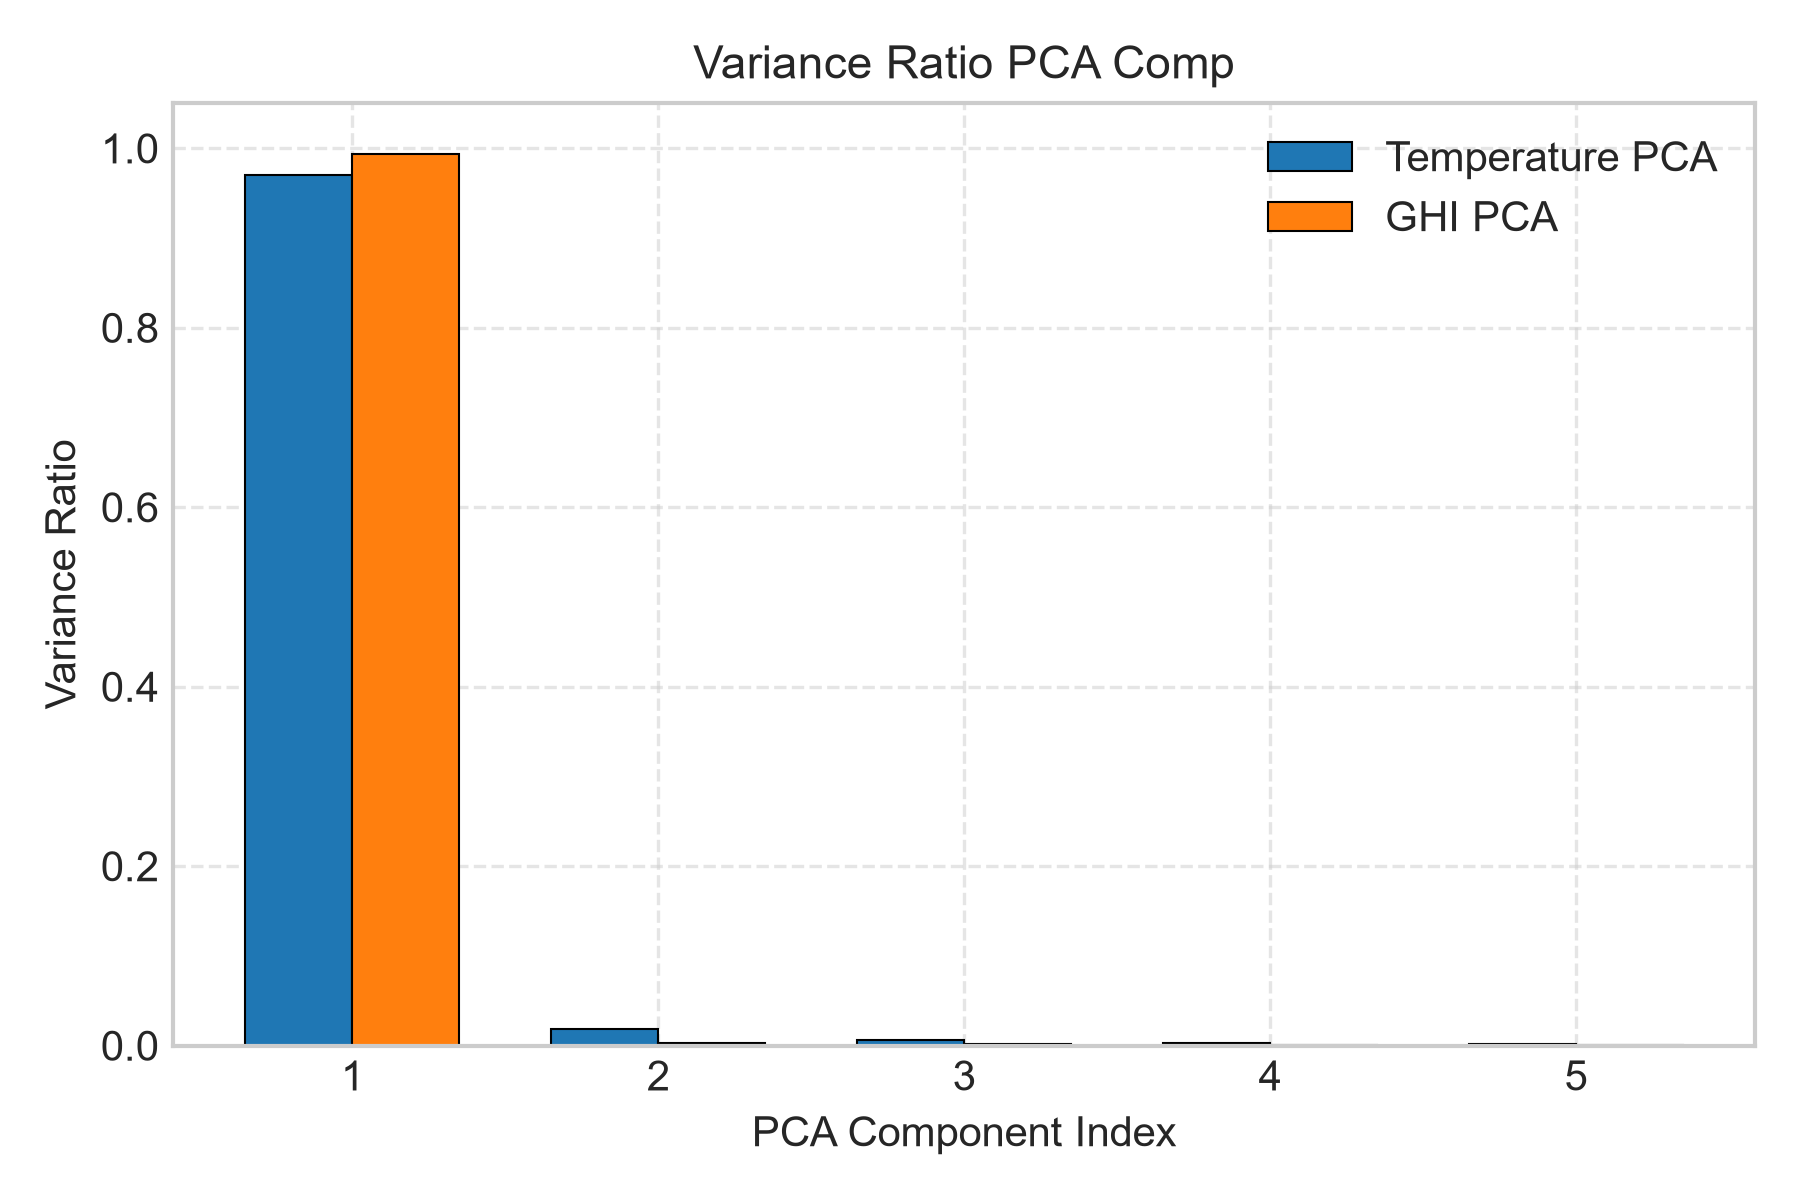
\includegraphics[width=0.75\textwidth]{figures/Figure_3_PCA_Components.png}
    \caption{Tỷ lệ phương sai giải thích của các thành phần chính PCA trên chuỗi Nhiệt độ và Bức xạ mặt trời GHI.}
    \label{fig:pca_variance}
\end{figure}

\subsubsection{2. Kỹ nghệ Đặc trưng Định hướng Vật lý}
Dựa trên tiêu chuẩn ASHRAE~\cite{ashrae2021fundamentals}, chúng tôi thiết lập hai chỉ số nhiệt động lực học tại nhiệt độ tiện nghi $T_{\text{base}} = 18.0^\circ\text{C}$:
\begin{align}
    \bar{T}_t &= \frac{1}{5} \sum_{i=1}^5 T_{i, t}, \quad \text{HDD}_t = \max\left(18.0 - \bar{T}_t, \; 0\right), \quad \text{CDD}_t = \max\left(\bar{T}_t - 18.0, \; 0\right)
\end{align}
Đồng thời, để loại bỏ bước nhảy gián đoạn của các biến giả tháng rời rạc, chuỗi điều hòa Fourier liên tục được thiết lập:
\begin{align}
    \text{Sin\_Year}_t &= \sin\left(\frac{2\pi \cdot \text{DOY}_t}{365.25}\right), \quad \text{Cos\_Year}_t = \cos\left(\frac{2\pi \cdot \text{DOY}_t}{365.25}\right) \\
    \text{Sin\_Hour}_t &= \sin\left(\frac{2\pi \cdot \text{Hour}_t}{24.0}\right), \quad \text{Cos\_Hour}_t = \cos\left(\frac{2\pi \cdot \text{Hour}_t}{24.0}\right)
\end{align}

\subsection{Cơ chế Đổi mới và Điểm Khác biệt so với Baseline}
Điểm đổi mới căn bản của kiến trúc Context-Aware Stacking (CAS) so với Stacking truyền thống của Wolpert~\cite{wolpert1992stacked} nằm ở việc \textbf{điều hòa meta-learner bằng vector ngữ cảnh môi trường thời gian thực}:
\begin{equation}
    \mathbf{z}_t = \Big[ \hat{y}_{\text{enet}, t}^{\text{OOF}}, \; \hat{y}_{\text{xgb}, t}^{\text{OOF}}, \; \mathbf{x}_{\text{context}, t} \Big]^T \in \mathbb{R}^{2 + d_{\text{ctx}}}
\end{equation}
trong đó $\mathbf{x}_{\text{context}, t} = [\text{Hour}_t, \text{HDD}_t, \text{CDD}_t, \text{Sin\_Year}_t, \text{Cos\_Year}_t, \text{PCA\_Temp}_t, \text{PCA\_GHI}_t, \dots]$.

\textbf{Giả thuyết cơ chế:} Trong khi mô hình Stacking truyền thống chỉ nhận vector dự báo tĩnh $[\hat{y}_1, \hat{y}_2]$ và bị "mù" thông tin thời gian thực, kiến trúc CAS cho phép meta-learner LightGBM hoạt động như một bộ định tuyến thích nghi động (\textit{adaptive dynamic router}): vào ban đêm khi phụ tải thuần baseload, mô hình tự động ưu tiên dự báo phẳng của ElasticNet; vào các buổi chiều hè nắng nóng khi CDD tăng vọt, mô hình chuyển dịch quyền quyết định sang cây XGBoost để bắt trọn phụ tải đỉnh.
